\documentclass[a4paper,10pt]{article}
\usepackage[utf8]{inputenc}
\usepackage{graphicx}
\usepackage{listings}
\usepackage{caption}
\usepackage{subcaption}
\usepackage{enumerate}

\usepackage{listings}
\usepackage[usenames,dvipsnames]{color}
\usepackage{courier}
\usepackage{fullpage}
\usepackage{url}


% Title Page
\title{}
\author{}


\begin{document}

\begin{titlepage}
\begin{center}


\textsc{\LARGE Royal Institute of Technology}\\[1.5cm]


%
\includegraphics[width=0.3\textwidth]{kth_mathematics_rgb.jpg}\\[1cm]
\begin{figure}[h]
        \centering
        \begin{subfigure}[b]{0.2\textwidth}
                \centering
                
\includegraphics[width=\textwidth]{kth_mathematics_rgb.jpg}
                \caption{Caroline}
                \label{fig:Caroline}
        \end{subfigure}%
        ~ %add desired spacing between images, e. g. ~, \quad, \qquad etc. 
          %(or a blank line to force the subfigure onto a new line)
        \begin{subfigure}[b]{0.2\textwidth}
                \centering
                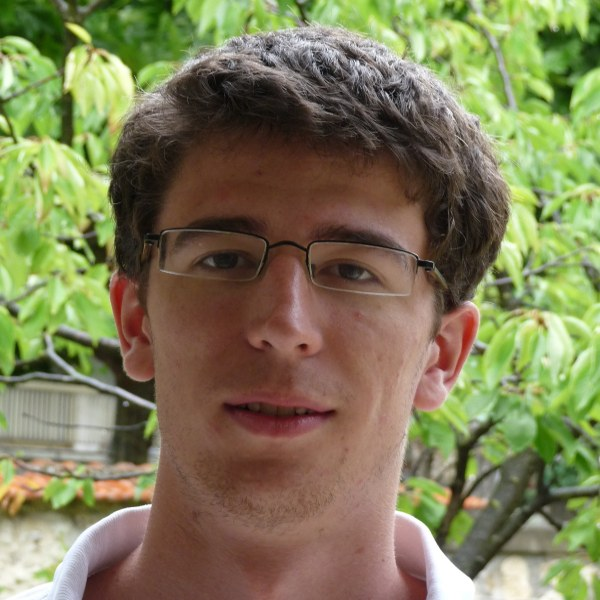
\includegraphics[width=\textwidth]{paul.jpg}
                \caption{Paul}
                \label{fig:Paul}
        \end{subfigure}
        \\ %add desired spacing between images, e. g. ~, \quad, \qquad etc. 
          %(or a blank line to force the subfigure onto a new line)
        \begin{subfigure}[b]{0.2\textwidth}
                \centering
                
\includegraphics[width=\textwidth]{sindri.jpeg}
                \caption{Sindri}
                \label{fig:Sindri}
        \end{subfigure}
          ~ %add desired spacing between images, e. g. ~, \quad, \qquad etc. 
          %(or a blank line to force the subfigure onto a new line)
        \begin{subfigure}[b]{0.2\textwidth}
                \centering
                
\includegraphics[width=\textwidth]{kth_mathematics_rgb.jpg}
                \caption{Tobias}
                \label{fig:Tobias}
        \end{subfigure}
        %\caption{Pictures of animals}\label{fig:animals}
\end{figure}

\textsc{\Large Artificial intelligence, dd2380 }  %\\ Instructor: Tobias Ryden , \emph{tryd@math.kth.se}}\\[0.5cm]

\hrulefill \\[0.4cm]
{ \huge \bfseries Final project: sokoban}\\[0.4cm]
\hrulefill \\[1.5cm]



    Caroline Laurène Kéramsi, keramsi@kth.se, XXXXXX-XXXX \\
    Paul Lagrée, lagree@kth.se, 900629-T133 \\
    Sindri Magnússon, sindrim@kth.se, 871209-7156 \\
    Tobias Johannes, Uebbing@kth.se, 900617-T251 \\


\vfill
% Bottom of the page
{\large \today}

\end{center}
\end{titlepage}


%%%%%%%%%%%%%%%%%%%%%%%%%%%%%%%%%%%%%%%%%%%%%%%%%%%%%%%%%%%%%%%%%%%%%%%%%%%%%%%%
%%%%%%%%%%%%%%%%%%%%%%%%%%%%%%%%%%%%%%%%%%%%%%%%%%%%%%%%%%%%%%%%%%%%%%%%%%%%%%%%
%%%%%%%%%%%%%%%%%%%%%%%%%%%%%%%%%%%%%%%%%%%%%%%%%%%%%%%%%%%%%%%%%%%%%%%%%%%%%%%%
%%%%%%%%%%
%%%%%%%%%% Report starts
%%%%%%%%%%
\cleardoublepage
\tableofcontents
\newpage

\abstract{ asdf}



\section{Introduction}

	\subsection{Problem description}
    Sokoban is a popular puzzle dating back to the eighties.  
    The original setting of the puzzle is a warehouse and the problem is to push boxes
    around to predefined storage locations.  
    But the underlying problem is of course much more abstract.  The rules are simple~\cite{wiki_soko}: 
    %cite http://en.wikipedia.org/wiki/Sokoban
    \begin{enumerate}[I]
        \item  Only one box can be pushed at a time.
        \item A box cannot be pulled.
        \item The player cannot walk through boxes or walls.
        \item The puzzle is solved when all boxes are located at storage locations.
    \end{enumerate}
    Even though the rules are simple, the problem is quite difficult and has been proven to be $NP$-hard.
    This is not only due to the branching factor but also the 
    enormous depth of the search tree~\cite{wiki_soko}.
    
    
    \subsection{Project organisation}
	We started with a simple implementation which was able to solve a small number of boards. 
	Then we applied different methods to improve it.
	As it takes time to get feedbacks from the server, we wrote our own bash script to evaluate the number of boards we are able to solve.
	This script runs our solver on 100 boards (server port 5032).
	We didn't want to wait too long for the results of the script so we limited the search time to 30 seconds per board.

\section{First version}
	\subsection{States representation}
	A state can be represented by the position of the player and the position of each boxes on the map. 
	Yet this representation is naive because it considers that states which differ only by a player move are different.
	For exemple the two following situations are considered as two different states even if we can go from one to the other only by moving the 
	player without touching a box.
	\begin{verbatim}
	#############                 #############
	#  .    $   #                 #  .    $   #
	#     @     #                 #@          #
	###$#########                 ###$#########
	#     $  ...#                 #     $  ...#
	#############                 #############
	\end{verbatim}
	

	We want to have a new state when we push a box and not when we move the player.
	So instead of considering the player position, we consider the area he can reach.
	This area can be computed easily by a recursive algortihm.
	The two situations can now be represented as the same state:
	\begin{verbatim}
	#############
	#XOOOOOO$OOO#
	#OOOOOOOOOOO#
	###$#########
	#     $  ...#
	#############

	O: reachable area
	X: leftest, upmost case of the reachable aread (called normalized position)
	\end{verbatim}
	Two states can be compared by looking at the box position and the leftest, upmost case of the reachable area.
	To avoid to save too many data, we destroy the reachable area when computed, and we keep only this normalized player position.

	
	\subsection{Search algorithm}
	To expand a state, we look at each direction of each box. 
	If a direction is inside the area that the player can reach, we look if there is a hindrance (box or wall) in the opposite direction.
	If this is not the case, the box can be pushed and we can create a new state.

	\begin{verbatim}
	#############  Here we can push down the leftest box because 
	#X .    $   #  the upper direction is inside the reachable 
	#  U        #  area and there is neither a wall nor a box
	###$#########  in the opposite direction
	#  D  $  ...#  
	#############  X: normalize player position

	We can create a new state:
	#############
	#X .    $   #
	#     @     #
	### #########
	#  $  $  ...#
	############# X: normalize player position
	\end{verbatim}

	The new state is compared with the states which have already been created. 
	If the state existed already, we delete the new state.
	Otherwise we add it to the list of created states and to the fifo of the states wich must be expanded.
	Then we can take the next state in the fifo and repeat the procedure.
	This is the Breadth-First-Search algorithm.

	\begin{figure}[h]
	\centerline{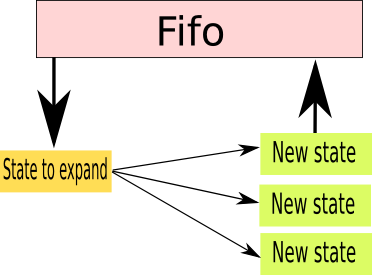
\includegraphics[height=5 cm, width=5cm]{./state_fifo.png}}
	\end{figure}

	We stop when we reach a final state (ie. a state where all the boxes are on a goal).
	Once we found a final state, we apply a pathfinding algortihm to build the solution string from the succession of states.

	\subsection{Pathfinding algorithm}

	The function findPath() in the class Ground will return the needed string containing the directions from the given start to 		the given goal. The function first checks whether the given start is not already the desired goal. In that case the function 		would just return an empty string. Otherwise findPath() calls it's helper function explorePath() that actual contains the 		pathfinding algorithm.

	The algorithm used within the explorePath() function is a directed DFS, that means it will dynamically try to go in the 	direction of the goal instead of always start to explore one specific direction. There will be more detailed explanation of 		this process later on.
	The explorePath() function first checks whether it has reached the aim. If that is true it returns. If not it tries to get a 		accessible neighbour point to go to using the getNextCell() function. If there is no suitable neighbour available the 		function returns the current point. So explorePath() ensures that the next cell to explore is not the current cell and then 		pushes the next cell on the end of the path point vector. Afterwards it calls itself recursivley with the next point as start 		and the the same goal as before.
	In the case there is no suitable neighbour to the current cell on the board explorePath() pushes the current cell to the 		daedends point vector which is used by the isPassable() function to make sure that the algorithm will not get to this board 		cell again. Then it calls itself recursivley again with the ancestor in the path point vector. 
	It can happen that the algorithm returns back to a path point and it came from the last possible move to make from that 	point. Than explorePath first removes this cell from the path point vector by testing whether the current cell is equal to 		the last path point saved in the path point vector before it does the recursive call.

	Next the functionality of the getNextCell() function will be described in more details, since it dymancially decides which 		direction is best to go to reach the goal as fast as possible. First getNextCell() calculates the distance of the x and y 		position of the goal to the ones of the aim. Then is tests which of the four directions is accessible and stores the result 		in an array. Then it decides which direction to go depending on the algebraic sign of the distance and whether this direction 		is passable. It has a preference to first go into the x direction and then in the y direction. If none of the prefered 		direction is suitable it attempts to choose the first passable direction within the passable array. If all that fails the 		return point stays the current point and the functions returns it.

	The isPassable() function that is used by the getNextCell function considers multiple situations that makes the point not 		passable. It takes into account whether the point was already visted before, is out of the board area, is blocked by a wall 		or a box or is a deadend that we have explored before.

	When the explorePath() function returns the findPath() function goes through the generated path point vector and generates 		the path string and returns it.

	A point of improvement would be to introduce a depth limit that is orientated on the manhattan distance to the goal and use 		iterative deepening. Additionally to reverse the order of the prefered dirctions and run the algorithm again before 		increasing the depth limit would improve the perfomance. But since this path finding algorithm effects the perfomance of the 		agent only very restricted the project team concentrated first on improving the solution finding algorithm.

	\subsection{Results}
	With this first version we could only solve 1 board out of 100. 

\section{Improvements}
    \subsection{Hash table for repeated states}
    To evoid to explore too many states, we decided to save all explored states. 
    When a state is created, we compare it to the already explored states. 
    If it has already been explored, then we do not add it to the fifo of states which will be explored. 
    By doing so, we expect to reduce the search space. 
    In the beginning, we used to save explored states in a simple list, but when we added a new state, we were obliged to scroll the whole list. 
    This linear time was a huge slow-down, so we decided to use another representation for explored states.
    
    Instead of using a simple list, we finally decided to use a hash table to represent them. 
    It permits to explore much more nodes in the tree since it runs much faster. 
    We do not scroll a whole list, but we compute a hash given the positions of boxes and the normalized player position. 
    We concatenate these parameters in a single string and compute the hash using an existing function for strings in the standard library.

	\subsection{Deadlocks}
	1 board solved (the same that with the initial algorithm) but the board is solved after around 3500 nodes (instead of 7700 before)

	It is not possible to go from all states to the final state.  
	For example if a box is blocked by a wall in both vertical and horizontal direction and is not located on a goal.  
	Since the box is stuck it can never reach a goal and hence it is not possible to go from this state to the final state.    
	We call such states deadlocks.

	\begin{verbatim}
	#############  The rightest box is stucked in a corner.
	#X .       $#  This state is a deadlock.
	#           # 
	###$######### 
	#     $  ...# 
	############# 
	\end{verbatim}

        Search in the subtree below a deadlock is just a waste since it is not possible to reach the final state from there.  
        It is therefore very desirable to be able to detect deadlock as soon as possible.
	  \subsubsection{Frozen deadlock}
	    We say that a box is frozen if it can neither be moved in horizontal nor vertical direction.  
	    A frozen box can sometimes be made un-frozen.  For example if the box is blocked by a box that is not frozen.  
	    Frozen deadlock occurs when a box is not located on a goal, frozen and can not be made un-frozen.  
	    A box can not be made un-frozen if it can not be moved in horizontal direction because of either:
	
	    \begin{enumerate}[I]
                \item There is a wall on either the left or right side of the box.
                \item There is a frozen box on either the left or right side of the box.
            \end{enumerate}
            and it can not be moved in vertical direction because either: 
            \begin{enumerate}[I]
                \item There is a wall either above or below the box.
                \item There is a frozen box either above or below the box.
            \end{enumerate}
            With these rules we can recursively check if a box causes a frozen deadlock.  
            The only problem is that we can get stuck in loop if some of the boxes in the recursion checks if the original box causes a frozen deadlock.  
            This can be avoided by treating all already checked box as a wall ~\cite{frozen_deadlock}.    
            The initial state should not contain a frozen deadlock.  
            For each new state after the initial state we check if the newly moved box is on goal and if not we check if it causes a frozen deadlock. 
            Even if the box is on goal the recursive algorithm could detect a frozen deadlock if the move freezes some other box that is not on a goal.  
            There was not enough time to implement this though.  The idea of the recursive algorithm is taken from  ~\cite{frozen_deadlock}.
          \subsubsection{Dead positions}
            There are some locations on the map such that if we put a box there it will always lead to a deadlock, we call those locations dead positions.  
            Some of these dead positions can easily be be found before we start the solver. 
            Then we just need to make sure that we don’t move boxes to these dead positions. 
            By doing that, we reduce a lot the search space since we remove many possibilities where we can push boxes.
            The dead positions types we detect are:
            \begin{verbatim}
	    ##           
	     #     #######        The box is stuck in a verical or horizontal line
	    $#     #  $  #        which contains no goals.
	     #            
	    ##         
	      
	      
	     #  #   #$   #       The box is stuck in both the vertical and horizontal
	    #$  $#   #  #$       direction not on a goal.
	    \end{verbatim}
            
            
	\subsection{Search algorithm}
	\subsubsection{A*}
	After having coded a simple BFS algorithm, we decided to improve it in an A* algorithm. 
	Instead of using a simple fifo for the states which still have to be explored, we sort them depending on a heuristic function. 
	This function compute the Euclidean distance (also know as 2-norm distance) of each  box to a goal. 
	Of course we do not use twice the same goal and we use the closest goal when it is possible. 
	This implementation has improved our Sokoban solver by reducing the number of nodes needed to be explored.

	\begin{figure}[h]
	\centerline{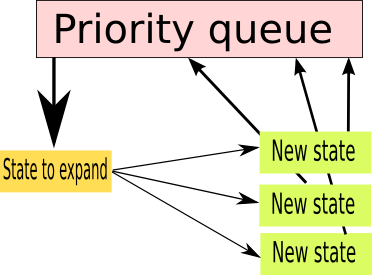
\includegraphics[height=5 cm, width=5cm]{./priority_state.png}}
	\end{figure}


    \subsection{Search}
        sdf~\cite{solving_soko}


\section{Results}

\section{Conclusions}
   
      
%%%%%%%%%%%%%%%%%%%%%%%%%%%%%%%%%%%%%%%%%%
%%%%%%%%%%%%%%%%%%%%%%%%%%%%%%%%%%%%%%%%%%
%%%%%%
%%%%%%  Appendix  
%%%%%%
%\appendix
 
%%%%%%%%%%%%%%%%%%%%%%%%%%%%%%%%%%%%%%%%%%
%%%%%%%%%%%%%%%%%%%%%%%%%%%%%%%%%%%%%%%%%%
%%%%%%
%%%%%%    
%%%%%% 
\bibliographystyle{plain} 
\bibliography{refs.bib}	
\end{document}          
